%%%%%%%%%%%%%%%%%%%%%%
%% Document details %%
%%%%%%%%%%%%%%%%%%%%%%

% Paper title
\title{Progress Report}

% Author
\author{Chris Cummins}

%%%%%%%%%%%%%%%%%%%%%%%%%
%% Document and Layout %%
%%%%%%%%%%%%%%%%%%%%%%%%%

% Fix for multiple "No room for a new \dimen" errors.
%
% See: http://tex.stackexchange.com/questions/38607/no-room-for-a-new-dimen
%
\usepackage{etex}

\usepackage{booktabs}

\usepackage[utf8]{inputenc}

% Make internal macro definitions accessible,
% e.g. \@title, \@date \@author.
\makeatletter

% Multi-column support.
\usepackage{multicol}

% A useful package which includes macros like \ifdef{}{}{}:
%
\usepackage{etoolbox}

% Uncomment the following line to remove column separation:
%
%\setlength{\columnsep}{5mm}


% Set chapter and section numbering depth:
%
\setcounter{secnumdepth}{2}


%%%%%%%%%%%%%%%%%%%%%%%%%%%%%%%%%
%% Bibliography and Appendices %%
%%%%%%%%%%%%%%%%%%%%%%%%%%%%%%%%%
\usepackage[%
    backend=biber,
    style=numeric-comp,  % numerical-compressed
    sorting=none,        % nty,nyt,nyvt,anyt,anyvt,ynt,ydnt,none
    sortcites=true,      % sort \cite{b a d c}: true,false
    block=none,          % space between blocks: none,space,par,nbpar,ragged
    indexing=false,      % indexing options: true,false,cite,bib
    citereset=none,      % don't reset cites
    isbn=false,          % print ISBN?
    url=false,           % print URL?
    doi=false,           % print DOI?
    natbib=true,         % natbib compatability
  ]{biblatex}

% Reduce the font size of the bibliography:
% \renewcommand{\bibfont}{\normalfont\scriptsize}

% Determine which BibTeX file to use:
%
% If available, use my Mendeley BibTex library, located in the home
% directory. Note that this is a relative path and will break if
% either this file or the BibTex library are moved. If the library is
% not present, use the local refs.bib file.
\newcommand{\BibResourceGlobal}{../../../../library.bib}
\newcommand{\BibResourceLocal}{refs.bib}

\IfFileExists{\BibResourceGlobal}
  {\newcommand{\BibResource}{\BibResourceGlobal}}
  {\newcommand{\BibResource}{\BibResourceLocal}}

\addbibresource{\BibResource}

% Appendix package. Documentation:
%
%  http://mirror.ox.ac.uk/sites/ctan.org/macros/latex/contrib/appendix/appendix.pdf
%
% Package options:
%
% toc      - Put a header (e.g., `Appendices') into the Table of Contents
%            (the ToC) before listing the appendices. (This is done by
%            calling the \addappheadtotoc command.)
% page     - Puts a title (e.g., `Appendices') into the document at the
%            point where the appendices environment is begun. (This is
%            done by calling the \appendixpage command.)
% title    - Adds a name (e.g., `Appendix') before each appendix title in
%            the body of the document. The name is given by the value
%            of \appendixname. Note that this is the default behaviour
%            for classes that have chapters.
% titletoc - Adds a name (e.g., `Appendix') before each appendix listed
%            in the ToC. The name is given by the value
%            of \appendixname.
% header   - Adds a name (e.g., `Appendix') before each appendix in page
%            headers.  The name is given by the value
%            of \appendixname. Note that this is the default behaviour
%            for classes that have chapters.
\usepackage[title, titletoc]{appendix}


%%%%%%%%%%%%%%%%%%%%%%%%%%%%%%%%%%%%%
%% Figures, footnotes and listings %%
%%%%%%%%%%%%%%%%%%%%%%%%%%%%%%%%%%%%%

%\usepackage{float}
%\restylefloat{figure}

% Use bold ``(Figure|Table|Listing)'' caption text.
%\usepackage[margin=1cm]{caption}

% Set the font for captions.
%\renewcommand{\captionfont}{\footnotesize}
% Set the font for caption labels.
%\renewcommand{\captionlabelfont}{\footnotesize\bf}

% Use arabic numbers for footnote.
%\renewcommand{\thefootnote}{\arabic{footnote}}

% Ensure that footnotes always appear at the bottom of pages.
%\usepackage[bottom]{footmisc}

% Reset the footnote counter on every page.
%\usepackage{perpage}
%\MakePerPage{footnote}

% Pre-requisites for rendering upquotes in listings package.
\usepackage[T1]{fontenc}
\usepackage{lmodern}
\usepackage{textcomp}

% Pseudo-code listings.
\usepackage{algorithm}
\usepackage{algpseudocode}
\newcommand{\Break}{\State \textbf{break} }
\algblockdefx[Loop]{Loop}{EndLoop}[1][]{\textbf{Loop} #1}{\textbf{End
    Loop}}

\algrenewcommand\ALG@beginalgorithmic{\footnotesize}

% Code listings.
\usepackage{listings}

% Set \ttfamily to use courier fonts.
%
% See: http://tex.stackexchange.com/a/33686
%
\usepackage{courier}

\lstset{frame=bt,                    % Add top and bottom frame lines
        breaklines=true,             % Force line wrapping
        captionpos=b,                % Place caption below listing
        numbers=left,                % Add left-side line numbers
        basicstyle=\scriptsize\ttfamily, % Set font size and type
        showstringspaces=false,      % Don't show visible whitespace
        numberstyle=\tiny,
        upquote=true,                % Use upright quotes, not curly
        commentstyle=\bfseries}      % Embolden comments

% Use (*@ @*) to escape LaTeX commands within listings.
\lstset{escapeinside={(*@}{@*)}}

% Add 10pt space between chapters in TOC listings entries:
%\let\Chapter\chapter
%\def\chapter{\addtocontents{lol}{\protect\addvspace{10pt}}\Chapter}

% Add JavaScript support to listings. See:
%
%     http://tex.stackexchange.com/a/89576
%
\lstdefinelanguage{JavaScript}{
  keywords={
    break,
    case,
    catch,
    catch,
    do,
    else,
    false,
    function,
    if,
    in,
    new,
    null,
    return,
    switch,
    true,
    typeof,
    var,
    while}
  keywordstyle=\bfseries,
  ndkeywords={
    boolean,
    class,
    export,
    implements,
    import,
    this,
    throw}
  ndkeywordstyle=\bfseries,
  sensitive=false,
  comment=[l]{//},
  morecomment=[s]{/*}{*/},
  morestring=[b]',
  morestring=[b]"
}

% Add Clojure support to listings. See:
%
%     http://alexott.blogspot.co.uk/2010/01/clojure-latex.html
%
\lstdefinelanguage{Clojure}{morekeywords={
    *,
    *1,
    *2,
    *3,
    *agent*,
    *allow-unresolved-vars*,
    *assert*,
    *clojure-version*,
    *command-line-args*,
    *compile-files*,
    *compile-path*,
    *e,
    *err*,
    *file*,
    *flush-on-newline*,
    *in*,
    *macro-meta*,
    *math-context*,
    *ns*,
    *out*,
    *print-dup*,
    *print-length*,
    *print-level*,
    *print-meta*,
    *print-readably*,
    *read-eval*,
    *source-path*,
    *use-context-classloader*,
    *warn-on-reflection*,
    +,
    -,
    ->,
    ->>,
    ..,
    /,
    :else,
    <,
    <=,
    =,
    ==,
    >,
    >=,
    @,
    accessor,
    aclone,
    add-classpath,
    add-watch,
    agent,
    agent-errors,
    aget,
    alength,
    alias,
    all-ns,
    alter,
    alter-meta!,
    alter-var-root,
    amap,
    ancestors,
    and,
    apply,
    areduce,
    array-map,
    aset,
    aset-boolean,
    aset-byte,
    aset-char,
    aset-double,
    aset-float,
    aset-int,
    aset-long,
    aset-short,
    assert,
    assoc,
    assoc!,
    assoc-in,
    associative?,
    atom,
    await,
    await-for,
    await1,
    bases,
    bean,
    bigdec,
    bigint,
    binding,
    bit-and,
    bit-and-not,
    bit-clear,
    bit-flip,
    bit-not,
    bit-or,
    bit-set,
    bit-shift-left,
    bit-shift-right,
    bit-test,
    bit-xor,
    boolean,
    boolean-array,
    booleans,
    bound-fn,
    bound-fn*,
    butlast,
    byte,
    byte-array,
    bytes,
    cast,
    char,
    char-array,
    char-escape-string,
    char-name-string,
    char?,
    chars,
    chunk,
    chunk-append,
    chunk-buffer,
    chunk-cons,
    chunk-first,
    chunk-next,
    chunk-rest,
    chunked-seq?,
    class,
    class?,
    clear-agent-errors,
    clojure-version,
    coll?,
    comment,
    commute,
    comp,
    comparator,
    compare,
    compare-and-set!,
    compile,
    complement,
    concat,
    cond,
    condp,
    conj,
    conj!,
    cons,
    constantly,
    construct-proxy,
    contains?,
    count,
    counted?,
    create-ns,
    create-struct,
    cycle,
    dec,
    decimal?,
    declare,
    def,
    definline,
    defmacro,
    defmethod,
    defmulti,
    defn,
    defn-,
    defonce,
    defprotocol,
    defstruct,
    deftype,
    delay,
    delay?,
    deliver,
    deref,
    derive,
    descendants,
    destructure,
    disj,
    disj!,
    dissoc,
    dissoc!,
    distinct,
    distinct?,
    do,
    do-template,
    doall,
    doc,
    dorun,
    doseq,
    dosync,
    dotimes,
    doto,
    double,
    double-array,
    doubles,
    drop,
    drop-last,
    drop-while,
    empty,
    empty?,
    ensure,
    enumeration-seq,
    eval,
    even?,
    every?,
    false,
    false?,
    ffirst,
    file-seq,
    filter,
    finally,
    find,
    find-doc,
    find-ns,
    find-var,
    first,
    float,
    float-array,
    float?,
    floats,
    flush,
    fn,
    fn?,
    fnext,
    for,
    force,
    format,
    future,
    future-call,
    future-cancel,
    future-cancelled?,
    future-done?,
    future?,
    gen-class,
    gen-interface,
    gensym,
    get,
    get-in,
    get-method,
    get-proxy-class,
    get-thread-bindings,
    get-validator,
    hash,
    hash-map,
    hash-set,
    identical?,
    identity,
    if,
    if-let,
    if-not,
    ifn?,
    import,
    in-ns,
    inc,
    init-proxy,
    instance?,
    int,
    int-array,
    integer?,
    interleave,
    intern,
    interpose,
    into,
    into-array,
    ints,
    io!,
    isa?,
    iterate,
    iterator-seq,
    juxt,
    key,
    keys,
    keyword,
    keyword?,
    last,
    lazy-cat,
    lazy-seq,
    let,
    letfn,
    line-seq,
    list,
    list*,
    list?,
    load,
    load-file,
    load-reader,
    load-string,
    loaded-libs,
    locking,
    long,
    long-array,
    longs,
    loop,
    macroexpand,
    macroexpand-1,
    make-array,
    make-hierarchy,
    map,
    map?,
    mapcat,
    max,
    max-key,
    memfn,
    memoize,
    merge,
    merge-with,
    meta,
    method-sig,
    methods,
    min,
    min-key,
    mod,
    monitor-enter,
    monitor-exit,
    name,
    namespace,
    neg?,
    new,
    newline,
    next,
    nfirst,
    nil,
    nil?,
    nnext,
    not,
    not-any?,
    not-empty,
    not-every?,
    not=,
    ns,
    ns-aliases,
    ns-imports,
    ns-interns,
    ns-map,
    ns-name,
    ns-publics,
    ns-refers,
    ns-resolve,
    ns-unalias,
    ns-unmap,
    nth,
    nthnext,
    num,
    number?,
    odd?,
    or,
    parents,
    partial,
    partition,
    pcalls,
    peek,
    persistent!,
    pmap,
    pop,
    pop!,
    pop-thread-bindings,
    pos?,
    pr,
    pr-str,
    prefer-method,
    prefers,
    primitives-classnames,
    print,
    print-ctor,
    print-doc,
    print-dup,
    print-method,
    print-namespace-doc,
    print-simple,
    print-special-doc,
    print-str,
    printf,
    println,
    println-str,
    prn,
    prn-str,
    promise,
    proxy,
    proxy-call-with-super,
    proxy-mappings,
    proxy-name,
    proxy-super,
    push-thread-bindings,
    pvalues,
    quot,
    rand,
    rand-int,
    range,
    ratio?,
    rational?,
    rationalize,
    re-find,
    re-groups,
    re-matcher,
    re-matches,
    re-pattern,
    re-seq,
    read,
    read-line,
    read-string,
    recur,
    reduce,
    ref,
    ref-history-count,
    ref-max-history,
    ref-min-history,
    ref-set,
    refer,
    refer-clojure,
    reify,
    release-pending-sends,
    rem,
    remove,
    remove-method,
    remove-ns,
    remove-watch,
    repeat,
    repeatedly,
    replace,
    replicate,
    require,
    reset!,
    reset-meta!,
    resolve,
    rest,
    resultset-seq,
    reverse,
    reversible?,
    rseq,
    rsubseq,
    second,
    select-keys,
    send,
    send-off,
    seq,
    seq?,
    seque,
    sequence,
    sequential?,
    set,
    set!,
    set-validator!,
    set?,
    short,
    short-array,
    shorts,
    shutdown-agents,
    slurp,
    some,
    sort,
    sort-by,
    sorted-map,
    sorted-map-by,
    sorted-set,
    sorted-set-by,
    sorted?,
    special-form-anchor,
    special-symbol?,
    split-at,
    split-with,
    str,
    stream?,
    string?,
    struct,
    struct-map,
    subs,
    subseq,
    subvec,
    supers,
    swap!,
    symbol,
    symbol?,
    sync,
    syntax-symbol-anchor,
    take,
    take-last,
    take-nth,
    take-while,
    test,
    the-ns,
    throw,
    time,
    to-array,
    to-array-2d,
    trampoline,
    transient,
    tree-seq,
    true,
    true?,
    try,
    type,
    unchecked-add,
    unchecked-dec,
    unchecked-divide,
    unchecked-inc,
    unchecked-multiply,
    unchecked-negate,
    unchecked-remainder,
    unchecked-subtract,
    underive,
    unquote,
    unquote-splicing,
    update-in,
    update-proxy,
    use,
    val,
    vals,
    var,
    var-get,
    var-set,
    var?,
    vary-meta,
    vec,
    vector,
    vector?,
    when,
    when-first,
    when-let,
    when-not,
    while,
    with-bindings,
    with-bindings*,
    with-in-str,
    with-loading-context,
    with-local-vars,
    with-meta,
    with-open,
    with-out-str,
    with-precision,
    xml-seq,
    zero?,
    zipmap
  },
  sensitive,
  alsodigit=-,
  morecomment=[l];,
  morestring=[b]"
}[keywords,comments,strings]


%%%%%%%%%%%%%%%%%%%%%%%%
%% Graphics and maths %%
%%%%%%%%%%%%%%%%%%%%%%%%
\usepackage{amsmath}

% Additional amsmath symbols, see:
%
% http://texblog.org/2007/08/27/number-sets-prime-natural-integer-rational-real-and-complex-in-latex/
%
\usepackage{amssymb}

\usepackage{graphicx}
\usepackage{mathtools}
\usepackage{tikz}
\usepackage{tikz-qtree}

% Provide bold font face in maths.
\usepackage{bm}

\usepackage{subcaption}
\expandafter\def\csname ver@subfig.sty\endcsname{}

% Define an 'myalignat' command which behave as 'alignat' without the
% vertical top and bottom padding. See:
%     http://www.latex-community.org/forum/viewtopic.php?f=5&t=1890
\newenvironment{myalignat}[1]{%
  \setlength{\abovedisplayskip}{-.7\baselineskip}%
  \setlength{\abovedisplayshortskip}{\abovedisplayskip}%
  \start@align\z@\st@rredtrue#1
}%
{\endalign}

% Define additional operators:
\DeclareMathOperator*{\argmin}{arg\,min}
\DeclareMathOperator*{\argmax}{arg\,max}

% Skeleton operators.
\DeclareMathOperator*{\map}{Map}
\DeclareMathOperator*{\reduce}{Reduce}
\DeclareMathOperator*{\scan}{Scan}
\DeclareMathOperator*{\stencil}{Stencil}
\DeclareMathOperator*{\zip}{Zip}
\DeclareMathOperator*{\allpairs}{All\,Pairs}

% Maths plots using pgfplots, see:
%
%     http://pgfplots.sourceforge.net/pgfplots.pdf
%
\usepackage{pgfplots}

% Gantt charts using pgfgantt, see:
%
%     http://www.ctan.org/pkg/pgfgantt
%
\usepackage{pgfgantt}

% Fix milestone aspect ratio by defining a custom element.
\newganttchartelement*{mymilestone}{
  mymilestone/.style={
    shape=diamond,
    inner sep=2pt,
    draw=black,
    top color=black,
    bottom color=black,
  }
}

% Tikz flowchart configuration.
\usetikzlibrary{shapes,arrows,shadows,fit,backgrounds}
\tikzstyle{decision} = [diamond,
                        draw,
                        text width=4.5em,
                        text badly centered,
                        node distance=3cm,
                        inner sep=0pt]
\tikzstyle{block}    = [rectangle,
                        draw,
                        text width=5em,
                        text centered,
                        node distance=3cm,
                        minimum height=4em,
                        inner sep=.2cm]
\tikzstyle{line}     = [draw, -latex']

% Add dirtree picture style, see:
%
%     http://tex.stackexchange.com/a/34268
%
\newcount\dirtree@lvl
\newcount\dirtree@plvl
\newcount\dirtree@clvl
\def\dirtree@growth{%
  \ifnum\tikznumberofcurrentchild=1\relax
    \global\advance\dirtree@plvl by 1
    \expandafter\xdef\csname dirtree@p@\the\dirtree@plvl\endcsname{\the\dirtree@lvl}
  \fi
  \global\advance\dirtree@lvl by 1\relax
  \dirtree@clvl=\dirtree@lvl
  \advance\dirtree@clvl by -\csname dirtree@p@\the\dirtree@plvl\endcsname
  \pgf@xa=0.33cm\relax
  \pgf@ya=-\baselineskip\relax
  \pgf@ya=\dirtree@clvl\pgf@ya
  \pgftransformshift{\pgfqpoint{\the\pgf@xa}{\the\pgf@ya}}%
  \ifnum\tikznumberofcurrentchild=\tikznumberofchildren
    \global\advance\dirtree@plvl by -1
  \fi
}
\tikzset{
  dirtree/.style={
    growth function=\dirtree@growth,
    every node/.style={anchor=north},
    every child node/.style={anchor=west},
    edge from parent path={(\tikzparentnode\tikzparentanchor) |- (\tikzchildnode\tikzchildanchor)}
  }
}

% UML sequence diagram macros, see:
%
%     https://code.google.com/p/pgf-umlsd/
%
% Options:
%
%     underline - Underline object names
%
\usepackage[underline=false]{pgf-umlsd}

% Support for SVG graphics.
%
% NOTE that you must pass the "--shell-escape" argument to pdflatex to
% compile. NOTE also that images *MUST* be placed within the graphics
% path.
\usepackage{svg}
\graphicspath{{img/}}

%%%%%%%%%%%%%%%%%%%%%%
%% Tables and lists %%
%%%%%%%%%%%%%%%%%%%%%%

%\usepackage{enumitem}
%\setenumerate{itemsep=0pt}

% Use no left margin for lists:
%\setlist{leftmargin=*}

\usepackage{longtable}

% Define column types L, C, R with known text justification and fixed
% widths:
\usepackage{array}
\newcolumntype{L}[1]{>{\raggedright\let\newline\\\arraybackslash\hspace{0pt}}m{#1}}
\newcolumntype{C}[1]{>{\centering\let\newline\\\arraybackslash\hspace{0pt}}m{#1}}
\newcolumntype{R}[1]{>{\raggedleft\let\newline\\\arraybackslash\hspace{0pt}}m{#1}}


%%%%%%%%%%%%%%%%%%%%%%%%%%%%%
%% Typesetting and symbols %%
%%%%%%%%%%%%%%%%%%%%%%%%%%%%%

% Adjustable font sizes in \Verbatim{}
\usepackage{fancyvrb}

%\usepackage{titlesec}
% Set section and paragraph heading fonts:
%\titleformat*{\section}{\Large\bfseries}
%\titleformat*{\subsection}{\normalsize\bfseries}
%\titleformat*{\subsubsection}{\normalsize}
%\titleformat*{\paragraph}{\large\bfseries}
%\titleformat*{\subparagraph}{\large\bfseries}

% Set section heading margins. Usage:
% \titlespacing*{<command>}{<left>}{<before>}{<after>}
%\titlespacing*{\section}{0pt}{.6em}{.3em}
%\titlespacing*{\subsection}{0pt}{.6em}{.2em}

% Set paragraph indentation size. Default is 15pt.
%\setlength{\parindent}{10pt}

% The line spacing can be globally set using \linespread:
%
% \linespread{1.2}

% Add a command \hr{} which will draw a horizontal rule the width of
% the text.
%
\newcommand{\hr}{\noindent\makebox[\linewidth]{\rule{\textwidth}{0.2pt}}}

% Add a command \br{} which will create a horizontal space of exactly
% one line height.
%
\newcommand{\br}{\hspace{\baselineskip}}

% Define a command to allow word breaking.
\newcommand*\wrapletters[1]{\wr@pletters#1\@nil}
\def\wr@pletters#1#2\@nil{#1\allowbreak\if&#2&\else\wr@pletters#2\@nil\fi}

% Define a command to create centred page titles.
\newcommand{\centredtitle}[1]{
  \begin{center}
    \large
    \vspace{0.9cm}
    \textbf{#1}
  \end{center}}

% Support hyperlinks using the \hyperref, \url and \href
% macros. Usage:
%
%    \hyperref[label_name]{''link text''}
%
%    \url{<my_url>}
%
%    \href{<my_url>}{<description>}
%
\usepackage{hyperref}

% Disable colored borders of links, cross-references etc in PDF output
\hypersetup{pdfborder={0 0 0}}

% Provide generic commands \degree, \celsius, \perthousand, \micro
% and \ohm which work both in text and maths mode.
\usepackage{gensymb}

%%%%%%%%%%%%%%%%%%%%%%%%%%%%%%%%%
%% Placeholder text generation %%
%%%%%%%%%%%%%%%%%%%%%%%%%%%%%%%%%

% Use either \blindtext or \libpsum to generate placeholder text. Also
% note the macros \blinditemize, \blindenumerate, \blinddescription.
\usepackage[english]{babel}
\usepackage{blindtext}
\usepackage{lipsum}


%%%%%%%%%%
%% Body %%
%%%%%%%%%%
\begin{document}

\maketitle

\begin{abstract}
  \noindent
  By their nature, Algorithmic Skeletons abstract implement details
  from the user which can be critical to performance. This project
  explores the effect of one such implementation detail --- setting
  the workgroup size of OpenCL kernels --- for SkelCL Stencil
  patterns. Through an exhaustive enumeration of a large optimisation
  space, we find that there is no one sensible default value which
  provides portable performance across the range of architectures,
  kernels, and datasets which SkelCL targets. As a result, we present
  a machine-learning enabled autotuner which performs runtime
  prediction of optimal workgroup sizes, achieving \todo{XXX}\%
  performance of the oracle, providing an average speedup of
  \todo{XXX}$\times$ (max \todo{XXX}$\times$) over the best statically
  chosen value.
\end{abstract}

\section{Introduction}
GPUs enable massive performance through heterogeneous
parallelism. However, developing software for these devices is
challenging, as the programming models provided by OpenCL and CUDA
require a low level knowledge of the underlying architecture to
properly exploit the potential performance. SkelCL addresses this
programmability challenge by providing high level skeleton patterns
for common data parallel operations. This project demonstrates that
the parameters which are necessarily abstracted by such skeletons can
have a huge impact on performance. To demonstrate this, I present an
autotuner for selecting the \emph{workgroup size} of Stencil pattern
kernels.

\section{Background}

In OpenCL, kernels are mapped to work-items for execution on the
processing units of GPUs and CPUs. These work-items are then grouped
into one or more workgroups. The choice of workgroup size is left to
the developer, but with two sets of constraints. The first set of
constraints is the maximum workgroup size which an execution device
supports. This value cannot be exceeded, irrespective of the kernel
being executed. The second constraint is the maximum workgroup size a
kernel supports, and can only be queried at runtime once a kernel has
been compiled. The selection of workgroup size for stencil skeletons
is particularly relevant to the performance of the stencil as it
affects utilisation of fast local memory. In a stencil code, each
work-item reads the values of multiple neighbouring elements. To
facilitate this, the value of all elements within a workgroup are
stored in fast local memory, which greatly reduces the read latency
for GPUs. Changing the workgroup size affects the amount of local
memory required for each workgroup, which in turn affects the number
of workgroups which may be simultaneously active.

\section{Methodology}

Tables~\ref{tab:hw},~\ref{tab:kernels}, and~\ref{tab:datasets} list
the range of execution devices, kernels, and datasets used. For each
unique combination of architecture, kernel, and dataset (hereby
referred to as a \emph{scenario}), training data was collected by
randomly sampling the space of legal workgroup sizes, until multiple
samples have been collected for each combination of scenario and
workgroup size.

\subsection{Oracle performance}
The arithmetic mean of the measured runtimes for a given scenario $s$
and workgroup size $w$ is represented by $t(s,w)$. The oracle
workgroup size for a given scenario is then the $w$ value from the set
of legal workgroup sizes $W$ which minimises the output of $t(s,w)$.

\[w_{oracle} = \argmin_{w \in W} t(s,w)\]

This allows relative comparisons of performance between different

For a given scenario $s$, the performance of workgroup size $w$ can be
compared relative to this oracle value.

\[p(s,w) = \frac{t(s,w_{oracle})}{t(s,w)}\]

These normalised comparisons of performance relative to the oracle can
be used by to provide an average performance for a given parameter $w$
across the set of all scenarios $S$.

\[\bar{p}(w) = \left(\prod_{s \in S} t(s,w_{oracle}) \cdot t(s,w)^{-1} \right)^{1/|S|}\]

\subsection{Autotuning}
The simplest autotuner is one which selects the workgroup size which
provided the best average case performance.

\[ \text{ZeroR} = \argmax_{w \in W} \bar{p}(w) \]

This provides a baseline for comparing against a more sophisticated
approach using machine learning. For each scenario, a feature vector
is extracted to capture properties of the architecture, device, and
dataset:

\begin{itemize}
\item \emph{Architectural features} --- size of local memory, maximum
  work group size, number of compute units, etc. Accessed using the
  OpenCL \texttt{clGetDeviceInfo()} API.
\item \emph{Kernel features} --- total static instruction count, ratio
  of instructions per type, ratio of basic blocks per instruction,
  etc. Accessed by compiling the OpenCL kernel to LLVM IR bitcode, and
  using the \texttt{opt} \texttt{InstCount} statistics pass.
\item \emph{Dataset features} --- size and type of the
  dataset. Accessed from the SkelCL Matrix container type.
\end{itemize}

See Appendix~\ref{app:features} for a full list of features and
types. For training, feature vectors are labelled with the oracle
workgroup size, and a machine learning classifier is trained on a
subset of this labelled training data. The performance of the
classifier can then be evaluated by comparing the performance of the
workgroup size predicted for an unseen feature vector against the
oracle workgroup size for that feature.

\subsubsection{Satisfying the maximum workgroup size constraint}

Since the space of legal workgroup sizes has hard constraints, it is
possible that a classifier will predict a workgroup size which
invalidates this constraint. To handle this situation, the workgroup
sizes predicted by the classifier are first checked to ensure that
they are less than or equal to the maximum workgroup size for that
scenario. If greater than, two strategies are evaluated:

\begin{enumerate}
\item Resorting to the ZeroR, i.e. the workgroup size which is known
  to be safe and provides the highest average case performance.
\item Incrementally reducing the workgroup size in each dimension
  until it falls within the space of legal workgroup sizes.
\end{enumerate}

\begin{table}
\footnotesize
\centering
\begin{tabular}{| L{1.2cm} | L{6.2cm} | L{1.5cm} | L{1.5cm} | L{1.5cm} | L{1.5cm} | L{1.5cm} |}
\hline
\scriptsize
\centering
\rowcolors{2}{white}{gray!25}
\begin{tabular}{ L{4.5cm} L{1.5cm} L{1.5cm} L{1.5cm} L{1.5cm} L{1.5cm} }
\hline
\scriptsize
\centering
\rowcolors{2}{white}{gray!25}
\begin{tabular}{ L{4.5cm} L{1.5cm} L{1.5cm} L{1.5cm} L{1.5cm} L{1.5cm} }
\hline
\scriptsize
\centering
\rowcolors{2}{white}{gray!25}
\begin{tabular}{ L{4.5cm} L{1.5cm} L{1.5cm} L{1.5cm} L{1.5cm} L{1.5cm} }
\hline
\input{gen/tables/devices}
\hline
\end{tabular}

\hline
\end{tabular}

\hline
\end{tabular}

\hline
\end{tabular}
\caption{%
  Execution devices. \TODO{I also have access to a machine with 4x GTX
    590 which I have yet to collect results for.}%
}
\label{tab:hw}
\end{table}

\begin{table}
\footnotesize
\centering
\begin{tabular}{| l | l | l | l | l | l |}
\hline
\scriptsize
\centering
\rowcolors{2}{white}{gray!25}
\begin{tabular}{lrrrrr}
\toprule
      Name &  North &  South &  East &  West &  Instruction Count \\
\midrule
   % complex &     30 &     30 &    30 &    30 &                161 \\
   % complex &      1 &     10 &    30 &    30 &                681 \\
   % complex &     20 &     10 &    20 &    10 &                161 \\
   % complex &      5 &      5 &     5 &     5 &                734 \\
   % complex &      5 &      5 &     5 &     5 &                161 \\
   % complex &      1 &     10 &    30 &    30 &                154 \\
   % complex &     10 &     10 &    10 &    10 &                161 \\
   % complex &     20 &     20 &    20 &    20 &                706 \\
   % complex &      1 &      1 &     1 &     1 &                137 \\
   % complex &     20 &     10 &    20 &    10 &                706 \\
   % complex &      1 &      1 &     1 &     1 &                661 \\
   % complex &     10 &     10 &    10 &    10 &                794 \\
   % complex &     30 &     30 &    30 &    30 &                706 \\
   % complex &     20 &     20 &    20 &    20 &                161 \\
   %  simple &      5 &      5 &     5 &     5 &                 67 \\
   %  simple &     20 &     10 &    20 &    10 &                612 \\
   %  simple &     20 &     20 &    20 &    20 &                612 \\
   %  simple &      1 &     10 &    30 &    30 &                592 \\
   %  simple &     10 &     10 &    10 &    10 &                700 \\
   %  simple &     30 &     30 &    30 &    30 &                612 \\
   %  simple &      1 &      1 &     1 &     1 &                 93 \\
   %  simple &     30 &     30 &    30 &    30 &                 67 \\
   %  simple &     20 &     10 &    20 &    10 &                 67 \\
   %  simple &      5 &      5 &     5 &     5 &                640 \\
   %  simple &     20 &     20 &    20 &    20 &                 67 \\
   %  simple &     10 &     10 &    10 &    10 &                 67 \\
   %  simple &      0 &      0 &     0 &     0 &                 40 \\
   %  simple &      1 &     10 &    30 &    30 &                 65 \\
   %  simple &      1 &      1 &     1 &     1 &                617 \\
   synthetic & 1--30 & 1--30 & 1--30 & 1--30 & 67--137\\
   synthetic & 1--30 & 1--30 & 1--30 & 1--30 & 592--706\\
   gaussian &      1--10 &      1--10 &     1--10 &     1--10 & 82--83 \\
  % gaussian &      5 &      5 &     5 &     5 &                655 \\
  % gaussian &      5 &      5 &     5 &     5 &                657 \\
  % gaussian &      0 &      0 &     0 &     0 &                 46 \\
  % gaussian &      5 &      5 &     5 &     5 &                 82 \\
  % gol &      1 &      1 &     1 &     1 &                714 \\
   gol &      1 &      1 &     1 &     1 &                190 \\
   he  &      1 &      1 &     1 &     1 &                113 \\
% he &      1 &      1 &     1 &     1 &                637 \\
%nms &      1 &      1 &     1 &     1 &                748 \\
   nms &      1 &      1 &     1 &     1 &                224 \\
%     sobel &      1 &      1 &     1 &     1 &               1008 \\
   sobel &      1 &      1 &     1 &     1 &                246 \\
% threshold &      0 &      0 &     0 &     0 &                 16 \\
   threshold &      0 &      0 &     0 &     0 &                 46 \\
\bottomrule
\end{tabular}

\hline
\end{tabular}
\caption{%
  Benchmark applications, border sizes, and static instruction counts.
  The ``simple'' and ``complex'' kernels are synthetic training
  programs. \TODO{I also have a FDTD benchmark which I have yet to
    collect results for.}%
}
\label{tab:kernels}
\end{table}

\begin{table}
\footnotesize
\centering
\begin{tabular}{| l | l | l | l |}
\hline
\footnotesize
\centering
\rowcolors{2}{white}{gray!25}
\begin{tabular}{ l l l l }
\hline
\footnotesize
\centering
\rowcolors{2}{white}{gray!25}
\begin{tabular}{ l l l l }
\hline
\footnotesize
\centering
\rowcolors{2}{white}{gray!25}
\begin{tabular}{ l l l l }
\hline
\input{gen/tables/datasets}
\hline
\end{tabular}

\hline
\end{tabular}

\hline
\end{tabular}

\hline
\end{tabular}
\caption{%
  Datasets used.%
}
\label{tab:datasets}
\end{table}

\section{Results}

A total of \input{gen/num_scenarios} scenarios were tested. For each
scenario, an average of \input{gen/num_avg_params} unique workgroup
sizes were tested (max \input{gen/num_max_params}), for a total of
\input{gen/num_runtime_stats} combinations of scenario and workgroup
size. For each of those, an average of \input{gen/num_avg_samples}
runtimes were collected (total
\input{gen/num_runtimes}). Figure~\ref{fig:max-wgsizes} shows the
distribution of maximum workgroup sizes across all
scenarios.

Figure~\ref{fig:oracle-wgsizes} shows the distribution of oracle
workgroup sizes. Clearly, the workgroup size $64 \times 4$.

Figure~\ref{fig:oracle-accuracy}


\begin{figure}
\begin{subfigure}[t]{0.45\textwidth}
\centering
\includegraphics{gen/img/max_wgsizes.png}
\vspace{-1.5em} % Shrink vertical padding
\caption{Maximum workgroup sizes}
\label{fig:max-wgsizes}
\end{subfigure}
~
\begin{subfigure}[t]{0.45\textwidth}
\centering
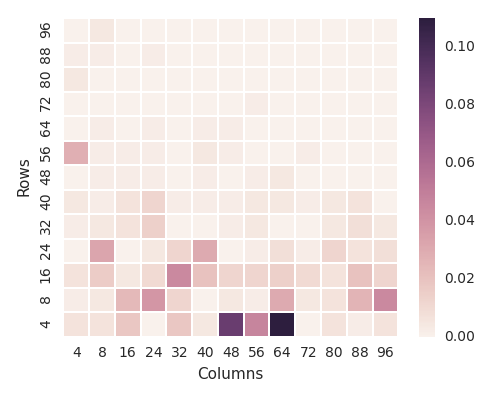
\includegraphics{gen/img/oracle_param_space.png}
\vspace{-1.5em} % Shrink vertical padding
\caption{Oracle workgroup sizes}
\label{fig:oracle-wgsizes}
\end{subfigure}
\caption{%
  On the left, the distribution of maximum legal workgroup
  sizes. Cells with a value of 1 indicate that the workgroup size is
  legal for all scenarios. A value of 0 shows a workgroup size which
  is illegal for all scenarios. On the right, the distribution of
  oracle workgroup sizes.%
}
\label{fig:heatmaps}
\end{figure}

\begin{figure}
\centering
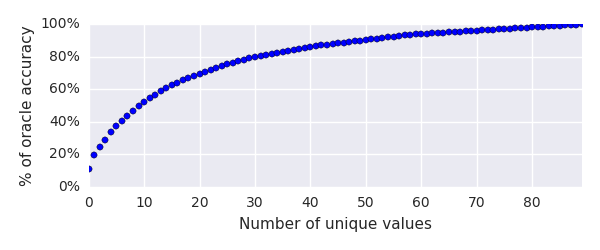
\includegraphics{gen/img/num_param_oracle.png}
\caption{%
  Accuracy compared to the oracle as a function of the number of
  workgroup sizes used. The best accuracy that is achievable using a
  single statically chosen value is 10\%.%
}
\label{fig:oracle-accuracy}
\end{figure}

\begin{figure}
\centering
\includegraphics{gen/img/params_summary.png}
\caption{%
  The blue line shows the performance of different workgroup sizes
  relative to the oracle. The green line shows the ``legality'' of the
  parameter value, i.e.\ the ratio of scenarios for which that
  workgroup size is legal.%
}
\end{figure}

\section{Evaluation}


\section{Conclusions}


\clearpage
\begin{appendices}

\section{Features}\label{app:features}

A full list of the feature names and types used to train machine
learning models. For training data, each feature vector was labelled
with the oracle workgroup size.

\begin{multicols}{2}
\begin{Verbatim}[fontsize=\footnotesize]
data_width                         numeric
data_height                        numeric
data_tin                           nominal
data_tout                          nominal
kern_north                         numeric
kern_south                         numeric
kern_east                          numeric
kern_west                          numeric
kern_max_wg_size                   numeric
kern_instruction_count             numeric
kern_ratio_AShr_insts              numeric
kern_ratio_Add_insts               numeric
kern_ratio_Alloca_insts            numeric
kern_ratio_And_insts               numeric
kern_ratio_Br_insts                numeric
kern_ratio_Call_insts              numeric
kern_ratio_FAdd_insts              numeric
kern_ratio_FCmp_insts              numeric
kern_ratio_FDiv_insts              numeric
kern_ratio_FMul_insts              numeric
kern_ratio_FPExt_insts             numeric
kern_ratio_FPToSI_insts            numeric
kern_ratio_FSub_insts              numeric
kern_ratio_GetElementPtr_insts     numeric
kern_ratio_ICmp_insts              numeric
kern_ratio_InsertValue_insts       numeric
kern_ratio_Load_insts              numeric
kern_ratio_Mul_insts               numeric
kern_ratio_Or_insts                numeric
kern_ratio_PHI_insts               numeric
kern_ratio_Ret_insts               numeric
kern_ratio_SDiv_insts              numeric
kern_ratio_SExt_insts              numeric
kern_ratio_SIToFP_insts            numeric
kern_ratio_SRem_insts              numeric
kern_ratio_Select_insts            numeric
kern_ratio_Shl_insts               numeric
kern_ratio_Store_insts             numeric
kern_ratio_Sub_insts               numeric
kern_ratio_Trunc_insts             numeric
kern_ratio_UDiv_insts              numeric
kern_ratio_Xor_insts               numeric
kern_ratio_ZExt_insts              numeric
kern_ratio_basic_blocks            numeric
kern_ratio_memory_instructions     numeric
kern_ratio_non_external_functions  numeric
dev_count                          numeric
dev_address_bits                   numeric
dev_double_fp_config               numeric
dev_endian_little                  numeric
dev_execution_capabilities         numeric
dev_extensions                     nominal
dev_global_mem_cache_size          numeric
dev_global_mem_cache_type          numeric
dev_global_mem_cacheline_size      numeric
dev_global_mem_size                numeric
dev_host_unified_memory            numeric
dev_image2d_max_height             numeric
dev_image2d_max_width              numeric
dev_image3d_max_depth              numeric
dev_image3d_max_height             numeric
dev_image3d_max_width              numeric
dev_image_support                  numeric
dev_local_mem_size                 numeric
dev_local_mem_type                 numeric
dev_max_clock_frequency            numeric
dev_max_compute_units              numeric
dev_max_constant_args              numeric
dev_max_constant_buffer_size       numeric
dev_max_mem_alloc_size             numeric
dev_max_parameter_size             numeric
dev_max_read_image_args            numeric
dev_max_samplers                   numeric
dev_max_work_group_size            numeric
dev_max_work_item_dimensions       numeric
dev_max_work_item_sizes_0          numeric
dev_max_work_item_sizes_1          numeric
dev_max_work_item_sizes_2          numeric
dev_max_write_image_args           numeric
dev_mem_base_addr_align            numeric
dev_min_data_type_align_size       numeric
dev_native_vector_width_char       numeric
dev_native_vector_width_double     numeric
dev_native_vector_width_float      numeric
dev_native_vector_width_half       numeric
dev_native_vector_width_int        numeric
dev_native_vector_width_long       numeric
dev_native_vector_width_short      numeric
dev_preferred_vector_width_char    numeric
dev_preferred_vector_width_double  numeric
dev_preferred_vector_width_float   numeric
dev_preferred_vector_width_half    numeric
dev_preferred_vector_width_int     numeric
dev_preferred_vector_width_long    numeric
dev_preferred_vector_width_short   numeric
dev_queue_properties               numeric
dev_single_fp_config               numeric
dev_type                           numeric
dev_vendor                         nominal
dev_vendor_id                      nominal
dev_version                        nominal
\end{Verbatim}
\end{multicols}

\end{appendices}

\end{document}
